% \documentclass[floatfix,nofootinbib,longbibliography,notitlepage]{revtex4-1}
\documentclass[floatfix,notitlepage]{revtex4-1}


%basic packages
\usepackage{xcolor}
\usepackage[T1]{fontenc}
\usepackage{hyperref}

\usepackage{amsthm}
\usepackage{amsmath}
\usepackage[mathscr]{euscript}
\usepackage{bbm}
\usepackage{times}
\usepackage{amsfonts}
\usepackage{amssymb}
\usepackage{thmtools}
%\usepackage{thm-restate}
%\usepackage{enumitem}
%\usepackage{amscd}
%\usepackage{graphicx}
%\usepackage{braket}
\usepackage{physics}
%\usepackage{multirow}
%\usepackage{tikz}
%\usetikzlibrary{quantikz}

\usepackage{graphicx}
\graphicspath{ {./figures/} }

% \usepackage[natbibapa]{apacite}

%colors
\definecolor{Fabulous}{RGB}{220,0,100}

%comments
\newcommand{\fm}[1]{{\color{Fabulous}\bf [FMM: #1]}}

\newcommand\numberthis{\addtocounter{equation}{1}\tag{\theequation}}

\def\textfmsy{$F_{\text{MSY}}$}
\def\fmsy{F_{\text{MSY}}}
\def\bmsy{B_{\text{MSY}}}

\def\bsurv{B_{\text{survey}}}
\def\vsurv{v_{\text{survey}}}
\def\nsurv{N_{\text{survey}}}
%
\def\vharv{v_{\text{harvest}}}
%
\def\ssb{\text{SSB}}

\def\obs{\text{obs}}

\def\eg{e.g.}


%handy macros
% eq + tab + enter: go to equation env
% align + tab + enter: similar but align env

\begin{document}
\title{When do size/age composition observations improve harvest control decisions?\\ A machine learning study on a spasmodic age-structured population}

\author{Felipe Montealegre-Mora}
\email{felimomo@berkeley.edu}
\affiliation{\
Department of Environmental Science, Policy and Management, University of California at Berkeley,  Berkeley, California, 94720, USA}
\affiliation{\ 
Eric and Wendy Schmidt Center for Data Science and Environment, University of California at  Berkeley, Berkeley, California, 94720, USA}

\author{Carl Boettiger}
\affiliation{\
Department of Environmental Science, Policy and Management, University of California at Berkeley,  Berkeley, California, 94720, USA}

\author{Carl J. Walters}
\affiliation{\
Institute for the Oceans and Fisheries, University of British Columbia, Vancouver, British Columbia, V6T 1Z4, Canada
}

\author{Christopher L. Cahill}
\affiliation{\
Quantitative Fisheries Center, Department of Fisheries and Wildlife, Michigan State University, East Lansing, Michigan, 48824, USA
}

\thanks{...
}

\date{\today}

\begin{abstract}
	In fishery science, harvest management of size-structured stochastic populations is a long-standing and  difficult problem. Rectilinear precautionary policies based on biomass and harvesting reference points have now become a standard approach to this problem. However, these policies are ultimately based on the theory of maximum sustainable yield and are theoretically grounded on the assumption that surplus production is stable in the fishery. This paradigm is challenged in fisheries with highly variable, spasmodic, recruitment. In this paper we explore the problem of designing harvest control rules for partially observed, age-structured, spasmodic fish populations using tools from reinforcement learning (RL) and Bayesian optimization. Our focus is on the case of Walleye fisheries in Alberta, Canada, whose highly variable recruitment dynamics have perplexed managers and ecologists. We optimized and evaluated policies using several complementary performance metrics. The main questions we addressed were: 1. How do standard policies based on reference points perform relative to numerically optimized policies? 2. Can an observation of mean fish weight, in addition to stock biomass, aid policy decisions? 
\end{abstract}

\maketitle

\tableofcontents
% so that the table of contents doesnt look weird:
\makeatletter
\let\toc@pre\relax
\let\toc@post\relax
\makeatother 

%
%
%
\section{Introduction}

Over the past two decades a wealth of literature has emerged that is aimed at solving sequential decision problems in diverse fields such as engineering, robotics, and control theory.  
This work, collectively referred to as Reinforcement Learning (RL), has now advanced to the level needed to outperform human experts in many fields~\cite{sutton-rl,bertsekas-rl}.  
For example, the application of RL has revolutionized games like chess, where the world’s top chess engines now almost always defeat the greatest chess players in the world. 
Beyond simply outperforming experts, RL offers a fresh perspective on previously unsolvable problems—and in the case of chess, top players now incorporate strategies discovered by engines into their own repertoires that were once considered nonsensical by humans. 
Lessons like these seem relevant to fisheries scientists, as a number of sustainability problems lie at the intersection of age-structured population dynamics and sequential decision making under uncertainty~\cite{walters-hilborn-1978}, and for which methods like dynamic programming or analytical approaches break down due to computational costs or scalability issues related to the “curse of dimensionality.”  
It is in these complex decision-making contexts that RL shows much promise, and might serve as a useful guide for improving our collective intuition surrounding the design of feedback policies.

In the absence of tractable analytical or dynamic programming solutions to feedback policy design in fisheries, simulation-based approaches like Management Strategy Evaluation (MSE) have emerged to evaluate trade-offs among alternative feedback policies or harvest control rules~\cite{punt-mse}.
In an MSE, analysts first specify policies to test a priori, and only after the specification of a policy set is simulation then used to quantify the relative performance of those policies against explicit objective(s).
While extensive application of the MSE approach has proved it to be a useful tool for informing harvest policy (\eg,~\cite{edwards2016-mse}), it remains fundamentally limited to select among the a priori policy set chosen by analysts.  
Phrased differently, if a particular policy is not included a priori due to a lack of creativity on behalf of analysts or perhaps due to the constraints of national legislation (\eg, see~\cite{dfo2006}), then it simply is not possible to learn whether some alternative harvest control rule might outperform those tested.  
In the context of feedback policy design this may be problematic, because feedback policy design is notoriously difficult, often counterintuitive, and because analysts typically limit themselves to 1-dimensional control rules based on stock biomass. 
	
The dynamics  of an age-structured population occurs in  high dimensional spaces, and thus in some situations it is possible for different states to correspond to the same total stock biomass.  
For example, in a standard  age-structured model, many small fish can have the same total biomass as a few large fish. Not surprisingly, managers might prescribe different management actions  in  these different contexts (see similar arguments in~\cite{hilborn2002}). 
This dimensionality problem makes it difficult  to specify policies to test a priori. 
While age-structure makes it difficult to specify good policies a priori, it also implies that  managers have access to more information than total biomass in many real-world situations. 
For instance, knowing the mean fish weight in addition to total stock biomass can help the manager distinguish between a population with many small fish and one with a population biased towards large fish. 
	
Fish populations with highly variable recruitment are some of the most perplexing systems to learn from and thus in which to inform fisheries management~\cite{hjort1914,caddy-gulland}, and thus might serve as a useful test case in which to explore the utility of RL for improving feedback policy design.  
In this paper we define highly variable recruitment to mean that a fish population exhibits infrequent large year classes of at least 10-50 times the long-term average recruitment level (see~\cite{caddy-gulland}).  
While by definition such events are rare in any one system, a cursory review of the literature reveals that these types of fluctuations occur with some regularity in fisheries throughout the world (\eg, see~\cite{fisch-etal-2019,licandeo-etal-2020}).  
For example, while better fisheries management practices helped rebuild Northeast Atlantic fish stocks, it appears that of the stocks that displayed the strongest recoveries, record large year classes occurred at low abundance that drove stock productivity upward and out of low, collapsed states (see~\cite{zimmermann2019improved}).  
Similarly, Atlantic Redfish Sebastes fasciatus stocks off the eastern coast of Canada exhibit spasmodic recruitment fluctuations that make the application of standard stock assessment techniques and MSE challenging~\cite{licandeo-etal-2020}.  
In inland systems, Walleye Sander vitreus in Lake Erie increased from low abundance due to a large recruitment event in 2003, and this cohort has continued to support the bulk of one of most economically valuable recreational fisheries in the world for nearly a decade~\cite{schmitt-vandergoot}.  
In each of these examples, large recruitment events had marked effects on both population status and the users who rely upon those populations; however, such events are almost always written off as “environmental effects” and are notoriously difficult to predict with the reliability needed to inform feedback policy design (see~\cite{punt2014, myers1998}).  
	
Little work has examined the implications of infrequent large recruitment events on the performance of feedback policies in age-structured populations, even though such policies are now considered the de facto standard for managing fisheries exploitation worldwide (\cite{silvar-viladomiu,free-etal-2023}; however see~\cite{licandeo-etal-2020}).
This is noteworthy because nearly all of the theoretical work underpinning harvest control rule or feedback policy design has assumed populations exhibit uncorrelated recruitment anomalies originating from standard, stationary statistical distributions (\cite{walters1975optimal,walters-hilborn-1978,reed1979optimal}; however see~\cite{parma1990experimental,hawkshaw2015harvest}). 
In this paper, we apply RL and Bayesian optimization to the problem of designing harvest control rules (HCRs) for partially-observed age-structured populations exhibiting highly variable recruitment dynamics (see Fig. 1a).  
Specifically, we use these tools to explore whether multi-dimensional control rules—particularly rules depending on the total stock biomass and the mean fish weight—can be helpful for managing age-structured, spasmodic recruiting, populations. 
We focus our case study on a recreational Walleye fishery managed via harvest lottery in Alberta, Canada (see~\cite{sullivan2003}), as recent work showed these populations recovered from collapse due in part to large positive recruitment anomalies~\cite{post-etal-2002,cahill2022}. 
We compare the policies obtained by numerical optimization with a rectilinear precautionary rule recommended by Canada~\cite{dfo2006}.  

We evaluate HCRs with three types of utility functions: total harvest (yield maximizing), a risk-averse utility that prioritizes interannual consistency in catch, and a trophy fishing utility in which only sufficiently large fish are valued by harvesters (see Fig. 1b). 
We optimize and evaluate four kinds of HCRs: 1) constant fishing mortality (\textfmsy), 2) a rectilinear precautionary rule derived from \textfmsy and $\bmsy$ (see~\cite{dfo2006}, Fig 1) for a visualization), 3) an unconstrained optimum rectilinear precautionary rule and 4) an HCR parametrized by a deep neural network using RL (see Fig. 1c).

Our findings are that:
\begin{enumerate}
\item With respect to total harvest, optimizing HCRs in classes 3 and 4 lead to considerable improvements over the simpler HCRs of classes 1 and 2. Here, in particular, the unconstrained rectilinear rule (HCR class 3) performed better than all other policies tested.
\item With respect to the risk averse utility, we observed a low performance of the constrained rectilinear policy (HCR class 2), while other HCR classes showed performances similar to each other.
\item With respect to both total harvest and the risk averse utility, our RL optimization indicates that the additional mean weight observation adds little value to the HCR, and in fact seems to hamper the RL algorithm convergence. 
\item With respect to the trophy utility function, the RL algorithm is able to advantageously use the additional mean weight observation, leading to considerably higher utility than all other HCRs we tested. 
\end{enumerate}

With respect to the trophy utility function, the RL algorithm is able to advantageously use the additional mean weight observation, leading to considerably higher utility than all other HCRs we tested. 
Through optimization we found policies that performed better than both \textfmsy and the DFO-recommended rectilinear rule. 
Second, that the \textfmsy control rule performs well with respect to the risk-averse utility—in this case, that control rule performed on par with the much more complicated HCR classes 3 and 4. 

Result 3. was rather surprising. 
Because of the complex stochasticity patterns in the model we considered, and because of the high dimensionality of our system, analytical optimality results used to inform simple HCR functional forms do not hold. 
We expected that because of this complexity, policies optimized over high-dimensional and expressive spaces would lead to improvements with respect to simple policies informed by analytical results on one-dimensional systems. 
Moreover, we expected that an additional observation on the size-structure of the population would yield valuable information for policy decisions. 
This, however, was not the case.

Result 4., in contrast to Result 3., shows that for utility functions with a strong dependence on size-structure, additional size-structure observations can allow for a better performance. 
Moreover, it demonstrates that RL can be a useful tool for optimizing HCRs when no good candidate for the functional form of the HCR is known a priori. 
The policy obtained by RL uses the combined information provided by the stock biomass and mean weight observations to more accurately time harvest pulses. Such pulse harvesting strategies have been shown to be optimal in other fishery scenarios~\cite{botsford1981,darocha2013}.

%
%
%
\section{Methods}

A collection of 15-30 walleye lakes in Alberta are managed using a Special Harvest License (SHL), which enables managers to assign a Total Allowable Catch (TAC) to limit harvest, and which is unique for inland recreational fisheries in North America.  
Presently, managers use an indicator-based approach to set TACs in any particular year based on standardized gill-netting surveys which occur in fall.  
However,~\cite{cahill2022} showed that harvestable surplus existed in many systems even though many management plans stated the goal of seeking to harvest  for maximum sustainable yield.  
Consequently, we seek to improve the scientific defensibility of this TAC allocation process in the Alberta SHL walleye program. 
To do so, we extended a standard age-structured population dynamics model of walleye described in detail in~\cite{cahill2022} and use it to simulate realistic population dynamics.  
Briefly, we model population processes such growth in numbers at age through time as a function of Beverton-Holt stock-recruitment (see below), von Bertalanffy somatic growth in length-at-age (see~\cite{cahill2020spatial}), and total mortality as an additive process assuming total instantaneous mortality Z is equal to instantaneous natural mortality M plus fishing mortality rates imposed by recreational harvesters and which is modulated by vulnerability at age.  
Unless stated otherwise parameter values for all relationships are drawn from average values estimated in~\cite{cahill2020spatial}.

\subsection{Population dynamics}

A key finding of~\cite{cahill2022} was that recruitment dynamics were highly variable and/or spasmodic (see also~\cite{caddy-gulland}). 
Thus, we model a Walleye fishery population using a discrete-time, age-structured stochastic model with 20 age classes $(B_1, ... ,B_{20})$. 
Recruitment is modeled via the Beverton-Holt equation,
\begin{align*}
    B_1(t+1) &= r_t \alpha \frac{\ssb_t}{1 + \beta \ssb_t} - H_{t,1},\\
    B_a(t+1) &= s (B_{a-1}(t) - H_{t,a-1}), \quad \text{for } 2 \leq a < 20, \numberthis\\
    B_{20}(t+1) &= s (B_{20}(t) + B_{19}(t) - H_{t,19}).
\end{align*}
Here, $H_{t,a}$ is the harvested biomass of fish in age class $a$, $\ssb_t$ is the spawning stock biomass (\cite{cahill2022}, Eq. 8), $\alpha$ and $\beta$ are describing juvenile survival as a function of $\ssb_t$ , and $r_t$ is a random variable used to modulate recruitment from the standard Beverton-Holt model to account for highly variable and spasmodic stochastic recruitment dynamics. 
We model $r_t$ as a Bernoulli random trial with $\text{Pr}=0.025$, and when this trial is “successful” we subsequently sample rt from a uniform distribution ranging from 10 to 30. 
Phrased differently, when the Bernoulli trial for a given year is successful we multiply the Beverton-Holt recruitment prediction by a random factor of 10-30 in accordance with the types of recruitment dynamics documented in~\cite{cahill2022}. 
When the Bernoulli trial is “unsuccessful,” on the other hand, we sample $r_t$ from a standard log-normal distribution like those commonly used to simulate variable recruitment (e.g., see~\cite{quinn-deriso}).

The harvested biomass was calculated as
\begin{align*}
    H_{t,a} = B_a(t) F_t \vharv(a),
\end{align*}
where $F_t$ is the instantaneous  fishing mortality and $\vharv(a)$ vulnerability-at-age to harvest and was calculated as
\begin{align}
    \vharv(a) = \frac1{1 + \exp(-(a-a_{hv})/a_sl)},
\end{align}
with $a_{hv}=5$, and $a_{sl}=0.5$. 
Notice that even for a high net fishing mortality rate, e.g. $F=1$, the actual fishing mortality rate enacted on young age classes remains low, which is a common assumption in many recreational fisheries settings (e.g., see~\cite{golden2022focusing}).

Simulations were run for 1000 time-steps in a heuristic attempt to capture the long-term effects of HCRs on population dynamics and performance criteria. 
Specifically, the expected number of large year classes (ie. ‘‘successful’’ Bernoulli trials for $r_t$ ) over a period of 1000 time-steps is 25, which was judged to be high enough to capture the dynamics arising from a particular HCR. 
Using the nomenclature from the RL literature, these 1000-timestep simulations are called \emph{episodes}.

\subsection{Observations}

We model observations by simulating a survey carried out by a management agency tasked with managing the fishery. 
These observations are subsequently used by the HCR to set a fishing mortality for a specific  time-step. 
We consider two types of observations. 
The first is an estimate of the stock biomass vulnerable to the management agency’s survey equipment,
\begin{align}
    \text{Stock. Biom. Obs.} = \bsurv = \sum_{a=1}^{20} B_a \vsurv(a),
\end{align}
where $\vsurv(a)$ models the vulnerability at age of the stock survey process (see \cite{cahill2022}, Eq. 15). 
A second observation we consider is the mean weight of fish in the survey,
\begin{align}
    \text{Mean Wt. Obs.} = \text{Stock. Biom. Obs.} / \nsurv,
\end{align}
where $\nsurv$ is the number of fish observed in the survey,
\begin{align}
    \nsurv = \sum_{a=1}^{20} \frac{B_a \vsurv(a)}{w_a},
\end{align}
and where $w_a$ is the average weight at age $a$.
Mean weight is easy for managers to observe and is important to consider in the context of spasmodically recruiting populations, since large recruitment events are correlated with dips in the mean weight of fish in the population.

Here we emphasize that the system is thus only partially observed~\cite{memarzadeh2019}-–-while the system dynamics unfold in the high-dimensional space defined by the biomass of each age class, the manager observes only a two-dimensional summary statistics (i.e. mean biomass, total biomass via standard monitoring surveys). 
It is worth noting that while the model dynamics are Markovian in the full state space, the dynamics of these two observed states are not, making this a so-called Partially Observed Markov Decision Process, or POMDP.  
This mathematical inconvenience significantly increases the technical difficulty  of finding an optimal solution using classical tools like dynamic programming, and, historically, the analysis of ecological POMDP problems has been restricted to much smaller models  (e.g., see~\cite{williams2022}).

\subsection{Utility models}

We consider three utility models. 
1. Total harvest utility: the utility at a timestep t is given by
\begin{align}
    U_t = \sum_{a=1}^{20} H_{a,t}
\end{align}
where $H_{a,t}$ is the biomass of size-class a harvested during timestep $t$. 
2. Risk averse utility: a hyperbolic additive risk-averse utility function (also known as ‘HARA utility’), 
\begin{align}
    U_t = \left(
    	\sum_{a=1}^{20} H_{a,t}
    \right)^\gamma,
\end{align}
where $\gamma=0.6$ parametrizes the risk-aversion. 
We note that this is similar to using the natural log of catches as is commonly done in MSE, where the specific risk aversion $\gamma$ is set to a clear value for clarity, and we note that this parameterization converges on total harvest utility as $\gamma\to1$.  
This way, stable harvests are preferred, and occasional large harvests contribute proportionally less to the utility. 
3. Trophy fishing utility: here, harvested fish only contribute to the utility if they are above a certain size (age) class, $a > a_{tr.}$,
\begin{align}
    U_t = \sum_{a=a_{tr.}}^{20} H_{a,t}.
\end{align}
In our results we use $a_{tr.}=10$.

We considered utility functions one and two because they represent commonly acknowledged goals of fisheries management, that is maximizing yield and stabilizing harvests, which are to some degree at odds with one another and represent high harvest rates (maximizing yield) or low, but consistent harvest rates (maximizing risk-averse utility; see also~\cite{walters-parma-1996,collie2021}).  
Moreover we included the trophy fishing function to explore how our analysis would change for more complex, size-dependent, utility functions. 
Size dependence can be particularly relevant in cases where machinery to process harvests only operates within certain ranges of fish sizes, or perhaps when anglers desire large trophy-sized fish rather than valuing fish of any size equally (e.g., see~\cite{murphy-willis-book}).

\subsection{Harvest control strategies}

Here we describe the classes of harvest control rules that we optimize and evaluate.

\textbf{FMSY.} 
In this strategy, the agent applies the same fishing mortality F for every timestep. 
(The name comes from \emph{maximum sustainable yield}, since in the case that utility is total harvest, the optimal value \textfmsy is the constant fishing mortality that leads to the highest long-term yield on average \cite{hilborn-walters-1992}.)

\textbf{Precautionary Policy.}
A piece-wise linear HCR determined by three parameters: 
two stock biomass reference points $x_1$, $x_2$  and the fishing mortality at high stock biomass,  $y_2$ . 
The HCR is given by the following equations:
\begin{alignat*}{2}
    F_t &= 0, \quad && \text{if } \bsurv(t) < x_1,\\
    F_t &= y_2 \left(\frac{\bsurv(t) - x_1}{x_2 - x_1}\right), \quad && \text{if } x_1 \leq \bsurv(t) \leq x_2, \numberthis\\
    F_t &= y_2, \quad && \text{if } \bsurv(t) > x_2.
\end{alignat*}
For a visual guide of this policy, see \cite[Fig.~1]{dfo2006}. 
In the literature, the parameters of this policy are fixed using the biomass at which the fishery maximizes average production, $\bmsy$, as a reference point. 
A common choice is $x_1=0.4 \bmsy$, $x_2=0.8 \bmsy$ and $y_2=\fmsy$. 
We call this specific realization of the HCR the \emph{constrained precautionary policy} (cPP). 
In contrast, when we refer to the precautionary policy whose parameters $x_1$, $x_2$, $y_2$ have been numerically optimized as the \emph{optimized precautionary policy} (oPP). 
We evaluate both of these HCRs.

We collectively refer to the three policy types described above as \emph{fixed policies}, in the sense that their functional form is fixed \emph{a priori}, before the optimization begins. 
The process of optimizing these fixed policies is loosely inspired by MSE, where several competing policies are evaluated using dynamic simulations \cite{punt-mse}.

\textbf{Reinforcement learning policy.} 
This type of policy uses a neural network to express the harvest control rule. 
We explore two cases: one where only the stock biomass observation is used, and one where an additional mean weight observation is used. 
Mathematically,
\begin{align}
    F_t = f_\theta(\obs_t)
\end{align}
where $f_\theta$ is a neural network with parameters $\theta$, and $\obs_t$ represent survey observations collected at time-step $t$. 

The neural network used was a 3-layer feed-forward network with layers of size 64, 32, 16. 
We chose this network structure by the following argument. 
First, 3-layer neural networks are known to be good approximators for piecewise linear functions~\cite{liang2016deep}—--thus the network would in principle be able to converge to the precautionary policy if it were optimal. 
Moreover, by trial-and-error, we noticed that decreasing subsequent layer sizes seemed to improve training. 
Finally, we deliberately chose relatively small layer sizes to reduce training time.\footnote{
As a comparison point, the default network structure used by \emph{stable baselines 3}, the Python package we used for RL computations, has two layers of 64 neurons each.
}
We emphasize, however, that all these choices on network structure were heuristic and not principled.

\subsection{Bayesian optimization of fixed policy controls}

We used the framework of Bayesian optimization in order to find optimal parameters for the fixed policy HCRs. 
A general introduction to this type of algorithm may be found on~\cite{frazier2018bayesian,head-skopt}. 
Bayesian optimization algorithms solve the problem of minimizing an unknown objective function $f$ which one can only query with some stochasticity, i.e. where instead of being able to compute $f(x, y, z, \dots)$ exactly, we are only able to compute $f(x, y, z, \dots)+r$, where $r$ is random. 
Thus, this type of algorithm is designed to be able to approximate a solution to the minimization problem
\begin{align}
    \mathrm{argmax}_{x,y,z,\dots} f(x,y,z,\dots)
\end{align}
even when one can only evaluate $f(x, y, z, \dots)$ ‘‘imperfectly.’’ 
These algorithms are most useful in scenarios where evaluating $f(x, y, z, \dots)$ is computationally expensive because they tend to require much fewer queries (i.e. evaluations of $f(x, y, z, \dots)$ at particular points) than brute force optimization approaches.

In our case, the arguments $(x, y, z, \dots)$ are the parameters in the HCR function. 
That is, for the precautionary policy, the arguments are $x_1$, $x_2$, $y_2$ , whereas for the \textfmsy policy, the only argument is the mortality rate $F$. 
We maximize the average utility obtained by a policy by optimizing over these parameters. 
For example, for the constant mortality mortality policy,
\begin{align}
    \fmsy = \mathrm{argmax}_F \mathbb{E}[U(F)],
\end{align}
where $U(F)$ is the utility obtained by simulating an episode using a constant mortality $F$. 
Note that $U(F)$ is thus a random variable since the dynamics are stochastic.

Because of our system's high stochasticity, evaluating the mean episode reward afforded by any policy requires taking the average of many episodes and in our case we used 200 episodes. 

We used the \emph{Gaussian process minimizer} algorithm from the \emph{scikit-optimize} package in Python to perform this optimization, and allowed the algorithm to evaluate the objective function at 70 different points. 
The number of points was chosen heuristically—it was high enough for the optimization to converge, but low enough to provide reasonable runtimes. 
Further details of how this optimization procedure is performed may be found in companion Jupyter notebooks.\footnote{
Found in \url{https://github.com/boettiger-lab/rl4fisheries/tree/main/notebooks}
}

\subsection{Harvest control via neural network: reinforcement learning optimization}

Here we give a small overview of the RL methods we used to optimize neural network policies. 
For a broader introduction to RL, its methods, and applications in quantitative ecology, see~\cite{lapeyrolerie-rl}.

Reinforcement learning is a class of strategies to approach \emph{sequential decision problems} in which a simulated \emph{‘‘agent’’} interacts with a simulated \emph{‘‘environment’’}. 
The agent here represents the decision-maker, who observes and acts on the environment. 
In the context of our paper, the environment is an age-structured model of the fish population, while the agent is a manager tasked with making a quota decision each year. 
In RL, the agent can be restricted to only observe partial information about the state of the environment. 
Here we consider observations of the total stock biomass and the mean fish weight.

The simulation is broken down into time-steps. 
At the beginning of each time-step, the agent prescribes an action that it applies to the environment. 
Subsequently, the environment changes its internal state due to this action, and outputs an observation and a reward back to the agent. 
The observation is used by the agent to take the next action. A visualization of this is shown in \cite[Fig.~1]{lapeyrolerie-rl}.

In the classic example of an Atari video-games, the agent fills in the role of the person playing the game, while the environment is the game itself.\footnote{
Atari video-game environments have established themselves as a benchmark with which to test RL algorithms. For more information on these environments, see \url{https://gymnasium.farama.org/environments/atari/}.
}
In the context of this work, one can think of the manager prescribing a TAC as the RL agent making decisions given some partially observable fish population (or environment).

We call \emph{training} the process by which the agent optimizes the values of the neural network weights $\theta$ (i.e., the process by which the RL algorithm optimizes the HCR). 
During training, the agent collects data on time-step interactions with the environment, slowly learning which actions to avoid given an observation, and which actions to encourage. 
This is done, in broad terms, using a variation of \emph{stochastic gradient descent}, which takes advantage of the fact that gradients can be efficiently computed on neural networks by using the technique of \emph{back propagation} (for an introduction to back propagation, see, e.g.,~\cite[Chapter~7]{rojas1996}.

A variety of algorithms exist for training RL agents, each with its strengths and drawbacks.
 Here we focus on the \emph{Proximal Policy Optimization} algorithm (PPO), which has been shown to perform well over a broad set of benchmark environments~\cite{schulman-ppo}. 
 It moreover has also been shown to have a strong performance in problems related to population dynamics~\cite{lapeyrolerie-rl,prettydarngood}.\footnote{
 We tested certain other RL algorithms, such as the \emph{Truncated Quantile Critics} (TQC) algorithm, as well. 
 However, we found it hard to match the performance of PPO. 
 Because of this, we do not include the analysis of policies obtained with these other algorithms here. 
 The companion source code allows the user to easily reproduce our analysis for PPO and other RL algorithms.
 }

 As mentioned, the neural networks we use in our results are rather modest in size—with only a few thousand parameters. 
 The training times were also modest, comprising 6 million time-steps, or a bit under two hours of training on a commercial GPU.


\subsection{Policy evaluation}

After optimizing each HCR, we simulated $n=500$ episodes and recorded the total utility received in each episode. 
Moreover, to get a more detailed comparison of the dynamics induced by each HCR, we simulated an additional episode where we recorded the stock biomass, mean fish weight and fishing mortality. 
To ease comparison between policies, we used the same time-series of stochastic deviations $\{r_t\}_{t=1,\dots,1000}$ across all of the latter set of simulations.

%
%
%
\section{Results}

We frame our results conceptually in Fig.~1.
In Table 1 we show the parameter values obtained for the optimized fixed policies. The episode utilities obtained by these policies are displayed in Table 2 and Fig. 2. 
With respect to total harvest, the control with highest utility was the optimized precautionary policy, and all other HCRs except for FMSY were within one standard deviation of its performance. 
With respect to HARA, the 1-observation RL policy was the highest performing control, and all other HCRs were within a standard deviation of its performance except for the 2-observation RL control. 
Finally, with respect to trophy fishing, we observed that the 2-observation RL policy performed significantly better than all other policies tested.

\begin{figure}[h!]
	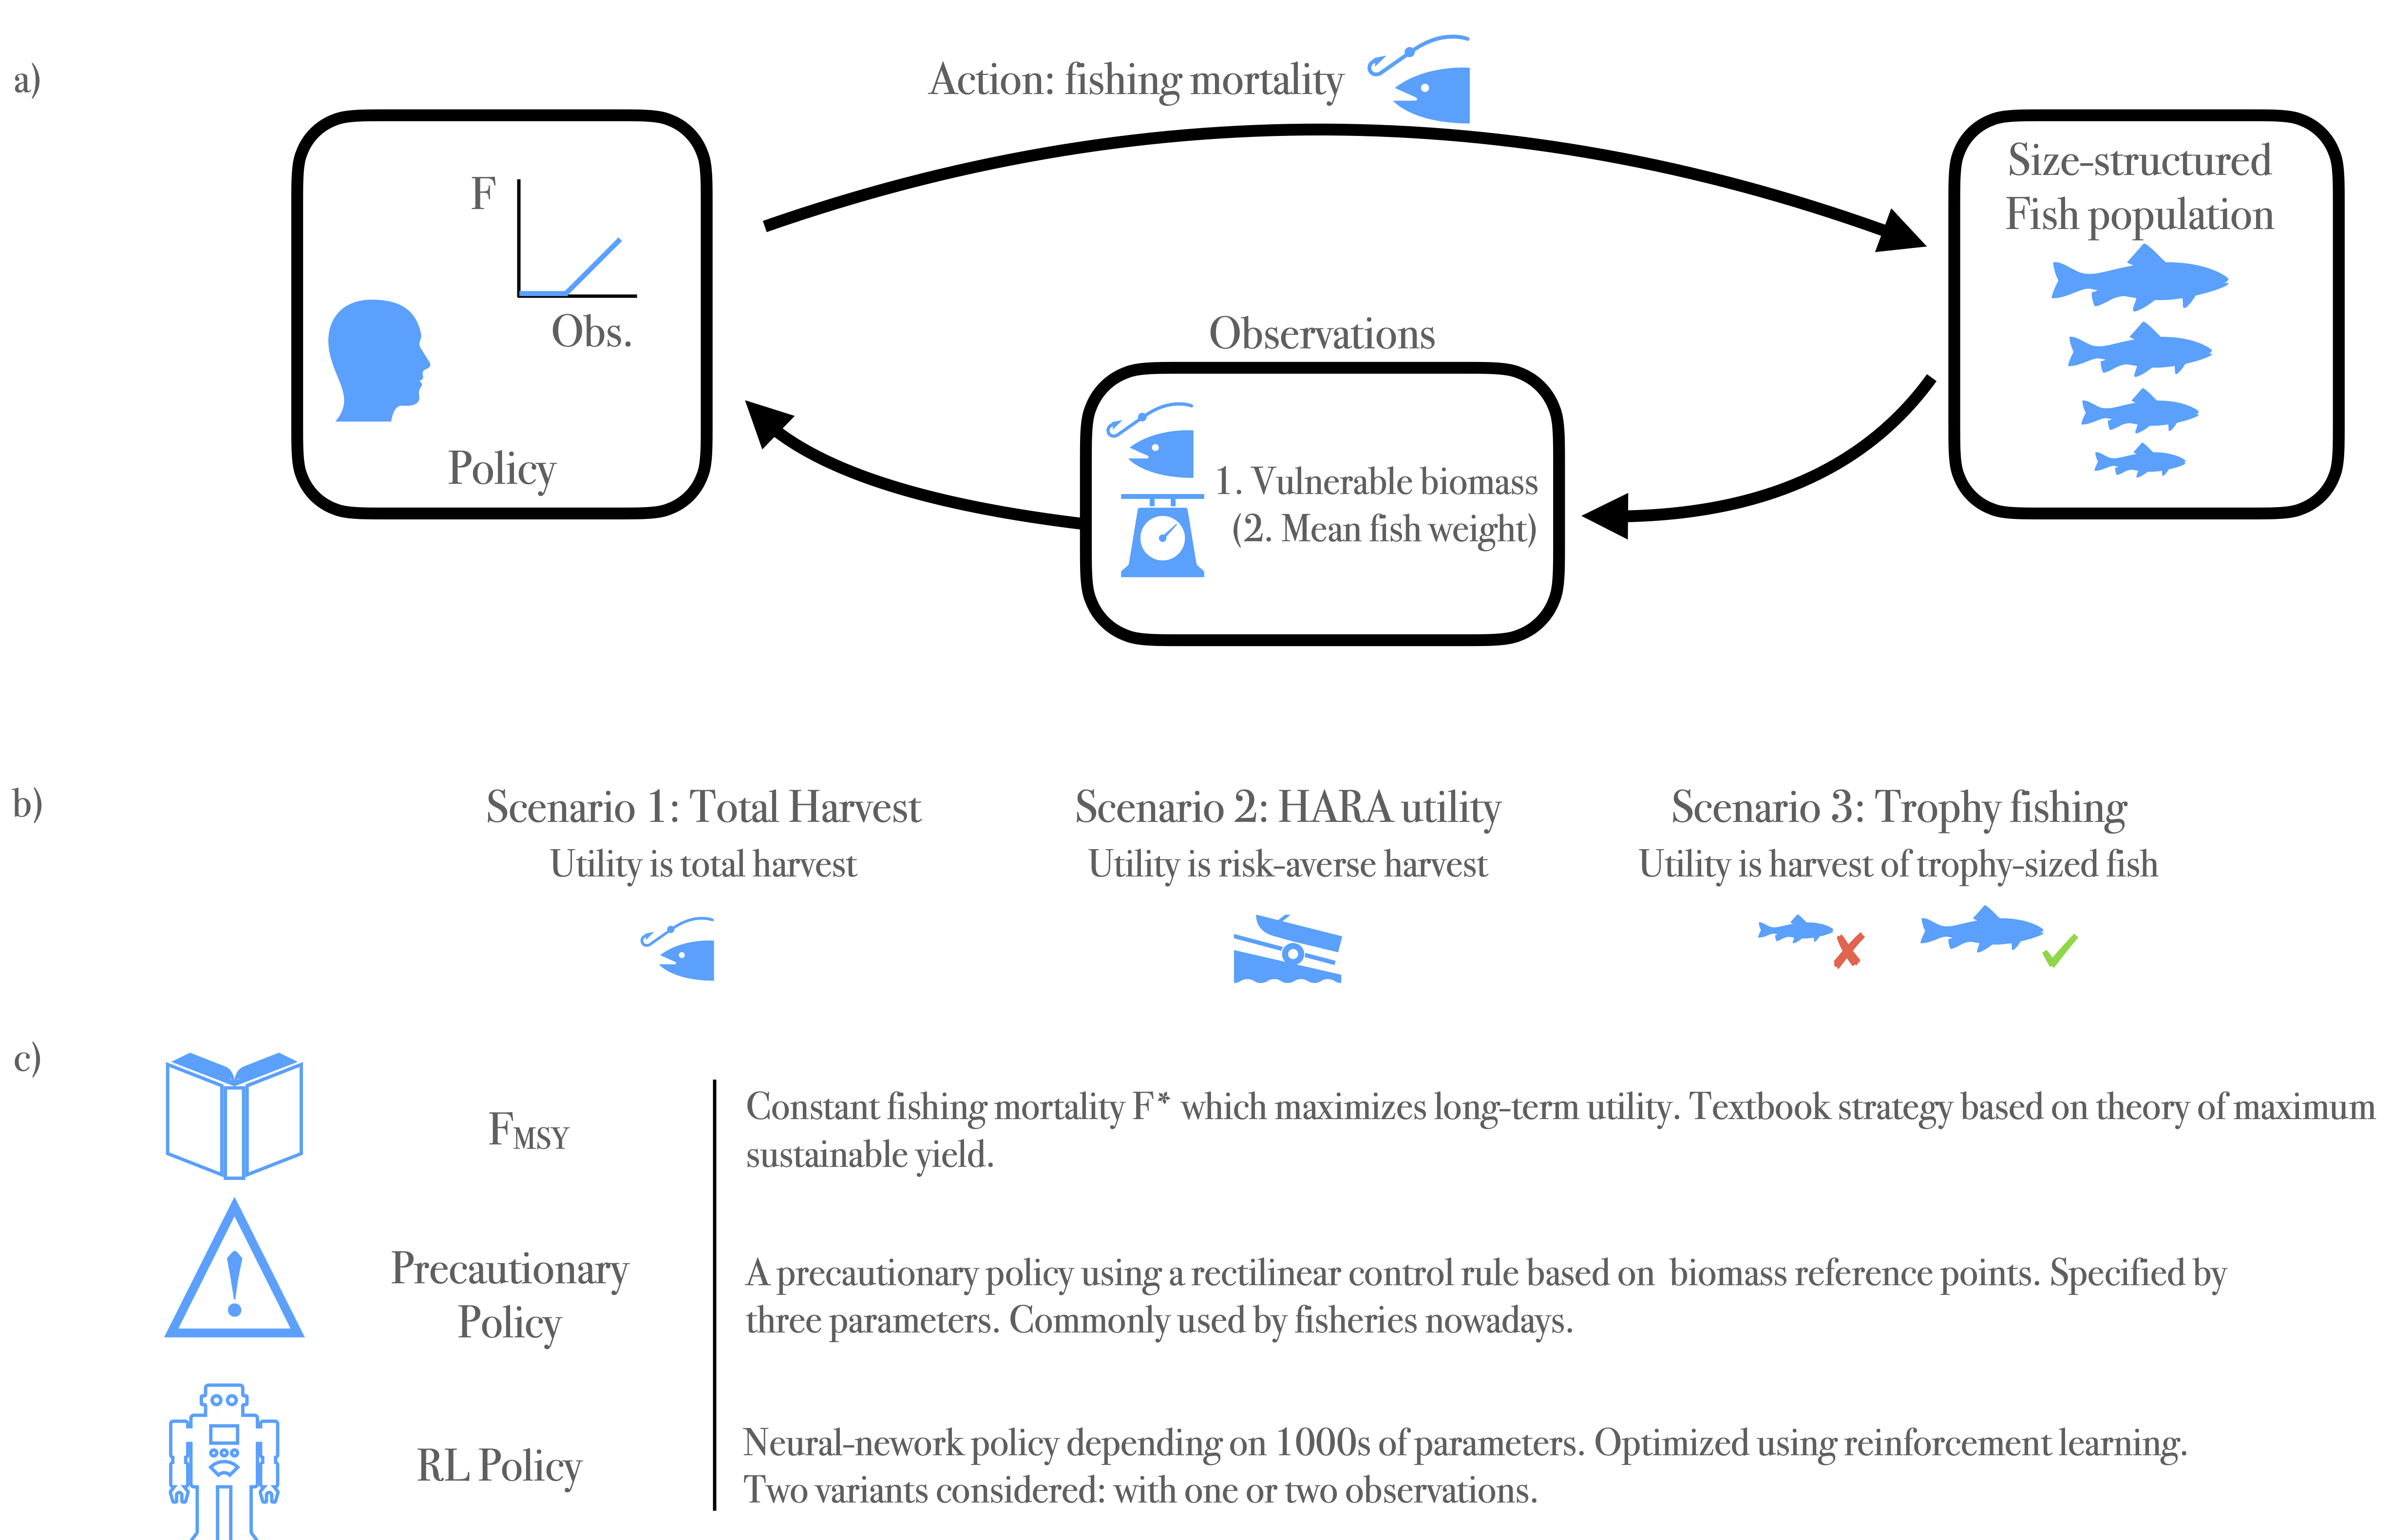
\includegraphics[width=.9\linewidth]{conceptual.png}
\caption{
\label{fig:conceptual}
Conceptual setting for our work.
}
\end{figure}



%
%
%
\section{Discussion}



%%%%%%%%%%%%%%%%%%%%%%%%%%%%%%%%%%%%%%%%%%%%%%%%%%%%%%%%%%%%%%%%%%%%%%%%%%%%%%%%%%%%%%%%%%

\bibliographystyle{unsrtnat} 
\bibliography{fishery_refs}



\end{document}
